\chapter{Traitement des données et classification}
Comme décidé lors de l'analyse de l'état de l'art et les réflexions de départ, la premières analyse qui est faite est de faire de la classification avant de tester les résultats de la régression. 

L'algorithme qui a été sélectionné pour effectué cette tâche est SVM (Support Vector Machines). Ce chapitre va décrire les différentes étapes qui ont été réalisée pour traiter les données et utiliser l'algorithme.

La programmation a été réalisée sur l'environnement PyCharm PROFESSIONAL 2019.2 et dans le langage Python. Cet environnement est le plus familier pour moi car il est étudié dans différents cours c'est pourquoi mon choix c'est porté sur ce dernier. 

%\begin{figure}[htp]
%	\begin{center}
%		
\includegraphics[scale=0.6]{figures/pycharm.png}
%		\caption{Logiciel utilisé pour le développement}
%		\label{fig:pycharm} %% NOTE: always label *after* caption!
%	\end{center}
%\end{figure}


\section{Structure du traitement}
Pour le traitement de données pour un apprentissage à l'aide d'un algorithme il est conseillé d'avoir différentes étapes voir Figure \ref{fig:process}. 

\begin{enumerate} 
	\item Acquisition des données : Étape délicate et très importante dans ce projet.
	\item Pré-traitement: Étape de traitement sur les données brutes se trouvant dans le set de données.
	\item Extraction des caractéristiques : Étape qui consiste à extraire les caractéristiques qui seront utilisée par l’algorithme pour faire la reconnaissance. 
	\item Reconnaissance : Utilisation d’un algorithme pour effectuer la reconnaissance des positions. 
	\item Décision :  Cette étape consiste, si cela est nécessaire, à décider du résultat final à l’aide d’une fusion, cela n'a pas été utilisé pour l'instant.
\end{enumerate}

\begin{figure}[H]
	\begin{center}
		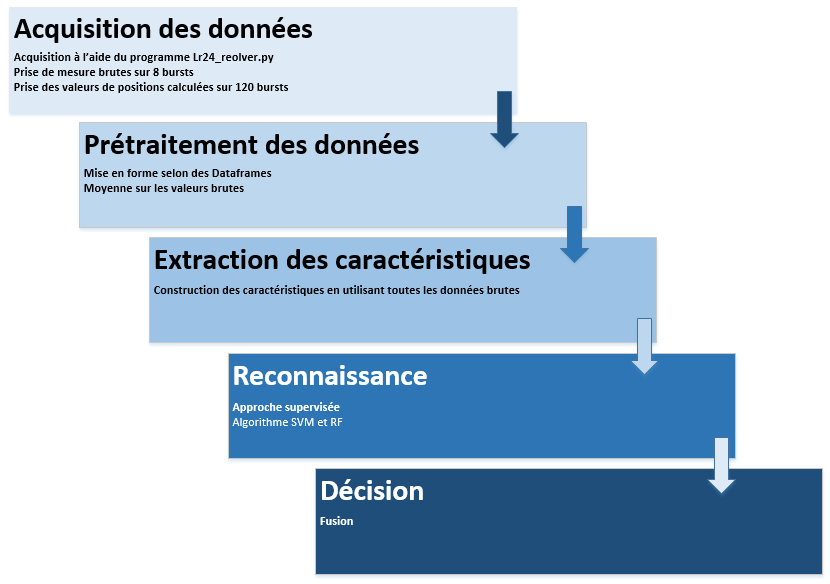
\includegraphics[scale=0.6]{figures/processing.png}
		\caption{Flux de traitement de l'information}
		\label{fig:process} %% NOTE: always label *after* caption!
	\end{center}
\end{figure}

Le premier point et l'acquisition de données qui est décrit au chapitre précédent. C'est une étape primordiale car c'est grâce à ces données que toute la suite de l'analyse va dépendre. Dans le cadre de ce projet, on remarque vite que si les données ne sont pas prises de manière rigoureuses, cela ne fonctionne pas.

Le pré-traitement consiste à utiliser les données disponible et de les exploiter. Dans un premier temps les données sont lue depuis un fichier *.npy qui représente des données NumPy. NumPy est une extension du langage de programmation Python, destinée à manipuler des matrices ou tableaux multidimensionnels ainsi que des fonctions mathématiques opérant sur ces tableaux. Plus précisément, cette bibliothèque logicielle libre et open source fournit de multiples fonctions permettant notamment de créer directement un tableau depuis un fichier ou au contraire de sauvegarder un tableau dans un fichier, et manipuler des vecteurs, matrices et polynômes \cite{WIKI2}. Depuis, ce fichier plusieurs traitement son effectué afin de transformer les données et les mettre dans un format permettant un traitement simple, le format "Dataframe" a été choisi et appartient à la librairie Pandas. Pandas est une bibliothèque écrite pour le langage de programmation Python permettant la manipulation et l'analyse des données. Elle propose en particulier des structures de données et des opérations de manipulation de tableaux numériques et de séries temporelles \cite{WIKI3}. A partir de là, il est possible d'utiliser les données afin d'en extraire des caractéristiques qui est l'étape suivante. Ce point sera détaillé plus loin afin de mieux comprendre ce qui a été utilisé pour que l'algorithme puisse au mieux reconnaitre les différentes positions. 

L'étape de reconnaissance consiste à entrainer un système avec les caractéristiques sélectionnées à partir des données et ensuite de valider que notre algorithme est capable de reconnaitre de nouvelles mesures. Ce point est également détaillé plus bas. 

Finalement, dans ce type d'analyse, il existe souvent une partie décision. Cela peut se faire car deux algorithme différents sont utilisées et il est nécessaire de décider quelle est le meilleur résultat. Dans le cadre de ce projet il n'a pas été nécessaire d'utiliser cela car il n'a pas été possible dans le temps imparti de tester plusieurs technique et donc la fusion n'était pas utile.

\section{Extraction des caractéristiques}
Ce chapitre traite des caractéristiques qui seront utilisées par l'algorithme afin de déterminer à quelle classe elles appartiennent. La Figue \ref{fig:dataframe} montre comment se présentent les données. Il est possible de les séparer et d'isoler chaque mesure. Chaque mesures est composée des données pour les quarante canaux (colonne : Canal).Les mesures qui peuvent être exploitées pour effectuer la classification est les mesures brutes de différence de distance (Sx.x). Il serait aussi possible d'exploiter la position fournie par le programme de prise de mesure mais cette dernière n'est pas assez représentative. C'est pour cette raison que deux type de classification ont été effectués. 

La première consiste à utiliser les données brutes et de travailler avec ces dernières pour extraire d'autres caractéristiques. Les principales qui ont été testée sont décrites ci-dessous.

\begin{enumerate}
	\item Toutes les données (raw) : Cela consiste à prendre toutes les mesures brutes de tous les canaux et de les mettre les unes après les autres. Ce qui veut dire que ca fait 320 valeurs (40 canaux fois 2x chaque esclave).
	\item Un canal (raw) : Cette façon de faire est identique à la précédente saut qu'un seul canal est pris en compte ce qui fait 8 valeurs (1 canal fois 2x chaque esclave).
	\item Moyenne : La moyenne est faite sur les 40 canaux par slave ce qui va donner huit caractéristiques supplémentaires.
	\item Variance : La variance est une mesure qui permet de caractériser la dispersion d'un échantillon. Elle est utilisée pour voir la dispersion des valeurs par esclave sur les quarante canaux. 
	\item Déviation standard : La déviation standard équivaut à la racine carrée de la variance. C'est donc une mesure de dispersion qui est faite également par esclave sur les quarante canaux. 
	\item Quantile : Un quantiles correspond à séparer les données en partie de taille égale. C'est-à-dire que chaque partie doit contenir le même nombre de données. Cela est également utilisé pour séparer les données au niveau des canaux pour un esclave.
	\item Médiane : La médiane est en quelque sorte le quantile qui sépare des données en deux partie de même taille. 
	\item covariance : La covariance permet de voir la corrélation entre des variables. Cette mesure est effectuée par esclave sur tous les canaux.  
\end{enumerate}
 
La deuxième consiste à utiliser uniquement la position fournie par le programme de prise de mesure. Cette position est mémorisée après avoir convergé et ce qui fait que les caractéristiques disponibles sont la coordonnée X et la coordonnée Y. Comme il n'y a que deux caractéristiques, il sera difficile d'effectuer différent traitement sur ces données si l'algorithme n'arrive pas différencier les classes. 

Les résultats de ces deux différentes approches seront détaillées au chapitre suivant. 

\begin{figure}[H]
	\begin{center}
		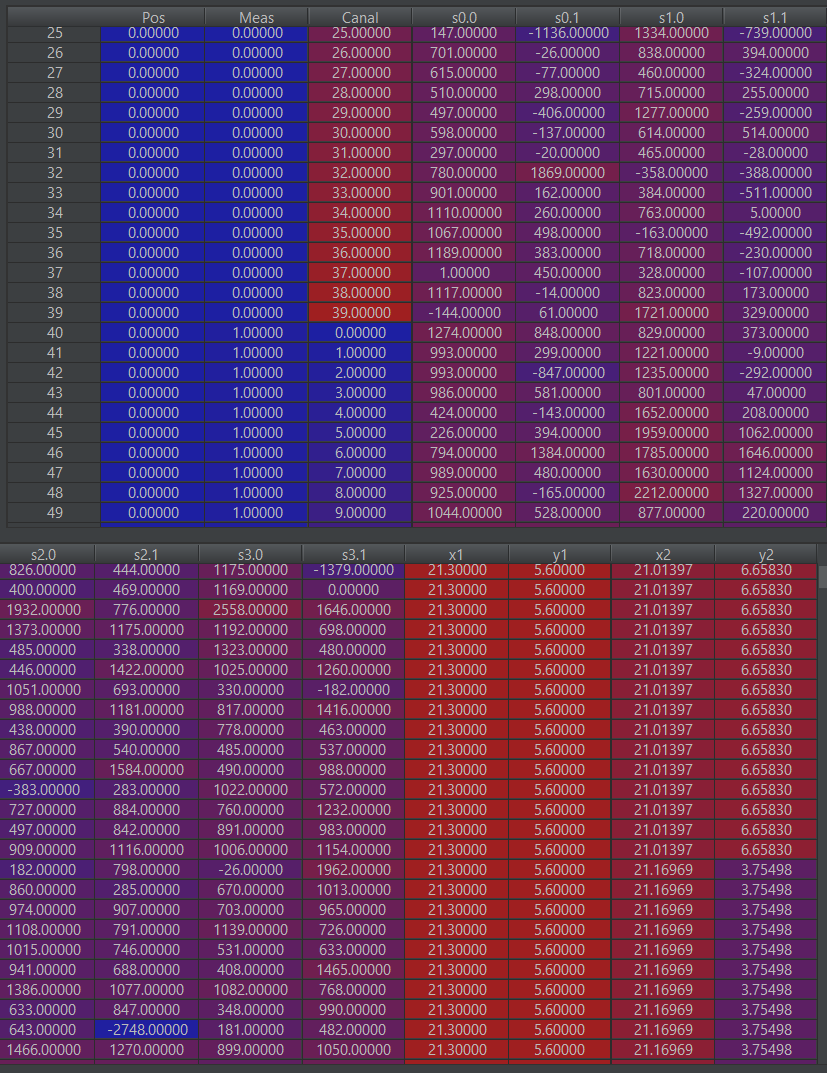
\includegraphics[scale=0.6]{figures/dataframe2.png}
		\caption{Données sous forme de dataframe pour le traitement et l'extraction des caractéristiques}
		\label{fig:dataframe} %% NOTE: always label *after* caption!
	\end{center}
\end{figure}

\section{Reconnaissance - Algorithme}
Le choix de l'algorithme utilisé a été fait par rapport à l'état de l'art qui a été effectué en début de projet. Comme déjà mentionné, l'algorithme qui a été retenu et SVM (Support Vector Machine). Cette solution permet de laisser le projet évoluer en utilisant dans un premier temps la solution pour la classification et ensuite en utilisant SVM pour la régression. 

Support vector machine est un algorithme supervisé qui permet de faire de la classification en essayant de trouver le meilleur hyperplan. La librairie scikit learn a été utilisée et je me suis servie de sklearn.svm.SVC (System Vector Classification).

L’implémentation de l’algorithme est facile une fois que les labels et les caractéristiques ont été extraits. Dans un premier temps, le canevas de base a été mis en place en utilisant les données brutes des mesures de "ranging". Cela a permis de faire les premiers réglages. 

Afin d'entrainer et de tester l'efficacité de l'algorithme il est nécessaire de partager les données en trois set. Il y a un set qui est utilisé pour l'entrainement, un set qui est utilisé pour valider l'entrainement qui vient d'être réalisé et un troisième set qui sert uniquement pour le résultat final. Dans ce dernier set, se sont des données que l'algorithme n'a jamais vu. La Figure \ref{fig:datasep} permet d'illustrer cette séparation. IL est également possible de voir que les données d'entrainement et de validation vont de pair. Pour ma part j'ai décidé d'effectuer une cross-validation. C'est-à-dire qu'à chaque lancement le partage des données n'est jamais identique. La seule chose qui est respectée est qu'il y aura toujours 20\% de données pour la validation et 80\% pour l'entrainement. Un autre chose qui est a vérifier c'est que les dataset soit balancé. Cela veut dire qu'il doit y avoir le même nombre de données de chaque classe dans chaque set. Cela donnerait de mauvais résultats si l'entrainement est fait avec les classes 1,2,et 3 et que la validation se fait avec des données des classes 4 et 5 par exemple. 

\begin{figure}[htp]
	\begin{center}
		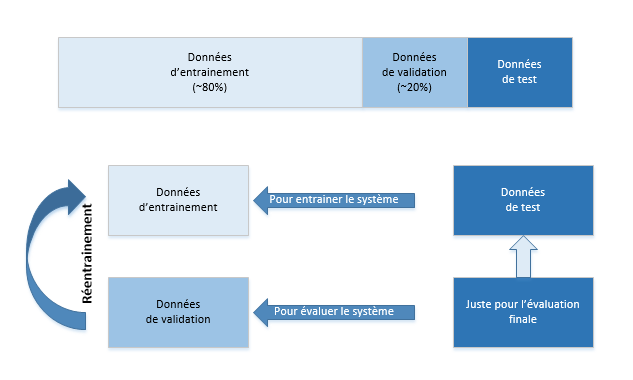
\includegraphics[scale=0.7]{figures/data_separation.png}
		\caption{Partage des données}
		\label{fig:datasep} %% NOTE: always label *after* caption!
	\end{center}
\end{figure}

\subsection{hyper-paramètres}
Il a été nécessaire de chercher les meilleurs paramètres pour SVM. Seul le kernel, le paramètre C et le paramètre gamma ont été cherchés. Une forte valeur de C tente de minimiser les erreurs de classification des données d'entraînement et une faible valeur essaie de maintenir une classification lisse. Concernant le gamma, plus il est grand , plus la cloche de la gaussienne est étroite voir Figure \ref{fig:c_gamma}. 

\begin{figure}[htp]
	\begin{center}
		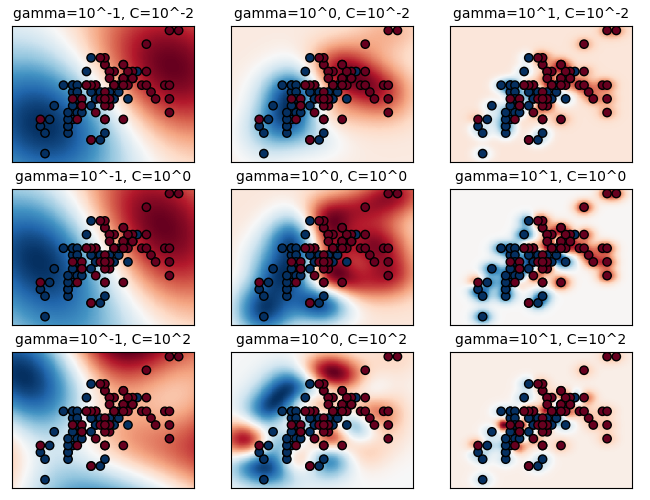
\includegraphics[scale=0.7]{figures/c_gamma_param.png}
		\caption{Influence des paramètres C et gamma}
		\label{fig:c_gamma} %% NOTE: always label *after* caption!
	\end{center}
\end{figure}

La première chose qui a été faite  a été de trouver le meilleur kernel pour cette classification. Dans mon cas, j’ai essayé les kernel suivant : linear, rbf, poly, sigmoid. Celui qui a donnée les meilleurs résultats et le kernel linear.

Suite à cela, un grid-search est effectué sur les paramètres C et gamma. Les meilleurs résultats obtenus pour la feature de la durée de charge sont avec un C égal à 100 et un gamma égal à 0.001. 

\section{Validation et résultats}
Cette section va présenter l'évolution des résultats obtenus au cours du développement. Voici un résumé des données acquises selon la Figure \ref{fig:mesures} : 

\begin{enumerate}
	\item Mesures de "ranging" effectuées sur les points Sx qui correspondent aux points que l'on souhaite retrouver (40x sur chaque point).
	\item Mesure de "ranging" effectuées sur les points Sx à un moment différent que les 40 mesures précédentes (5x sur chaque point).
	\item Mesure de "ranging" effectuées sur les points Tx. Ces points sont pris afin de voir si le plus proche voisin est retrouvé.
	\item Mesure de position effectuées sur les points Sx (40x + 5x sur chaque point).
	\item Mesure de position effectuées sur les points Tx (5x sur chaque point) 
\end{enumerate}

Ces différentes prises de données permettent de faire plusieurs analyses et comprendre de façon plus clair comment le système se comporte.

Les résultats sont évalués à l'aide des matrices de confusion mais également à l'aide de la mesure de précision, du F1-Score macro et finalement du F1-Score micro. 

La Figure \ref{fig:precisonrecall} montre ce que représente la précisoin et le rappel. Ces deux notions sont utilisées pour calucler le F1-Score de la manière suivante :

F1\_score = 2((Précision * rappel)/(Précision + rappel))

Le micro ou macro-avarage est utilisé pour analyser les données de manière différente. Pour le calcul du macro-avarage, il faut aditionner les précisions de chaque classe et le diviser par le nombre de classe. Dans ce cas il se pourrait qu'une classe soit très mauvaise et déséquilibrée mais que les autres remonte le score. Si maintenant on parle du micro-avarage, le calcule se fait en additionnat les vrais positif et en les divisant par le nombre total de point. Cette manière de faire va donner un score plus bas si une classe est déséquilibrée \cite{DATASCI}. 

Dans le cadre de cette analyse, toutes les classes possèdent le même nombre de données.

\begin{figure}[htp]
	\begin{center}
		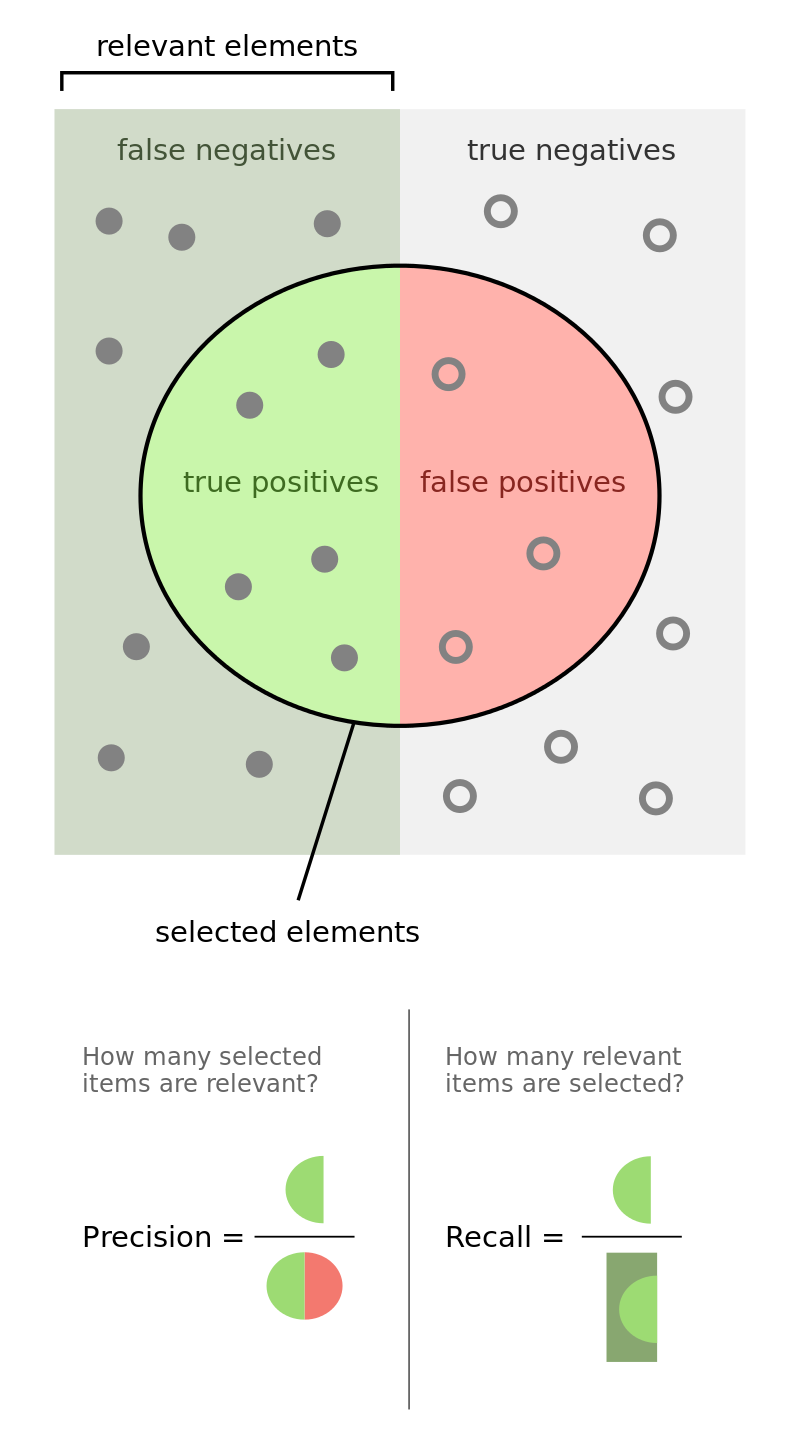
\includegraphics[scale=0.3]{figures/precisionrecall.png}
		\caption{Repérsentation de la précision et du rappel \cite{WIKI}}
		\label{fig:precisonrecall} %% NOTE: always label *after* caption!
	\end{center}
\end{figure}

\subsection{Résultats en utilisant les données de "ranging"}
Ce chapitre va présenter les résultats qui ont été obtenus à partir des données brutes de "ranging" fournies par le programme de mesures. Plusieurs traitements sont faits sur ces mesures afin d'améliorer les résultats. Le calule de position est également disponible mais n'est pas très représentatif car calculé uniquement à partir de huit valeurs de ranging (deux sur chaque esclave).


Afin d'avoir une meilleure vue de ce que représente les positions calculées sur peu d'échantillon, la Figure \ref{fig:plotPos} montre le positionnement de ces points calculés par rapport à la position réelle de l'espion. Les gros points de couleurs représentent la position réelle et les petits points de couleurs représentent les positions calculées. La croix noir représente la position du master. On remarque que les petits points sont bien plus espacés que lorsque l'on laisse converger la position (Figrure \ref{fig:plotPosConv}) mais il y a tout de même une séparation.

\begin{figure}[htp]
	\begin{center}
		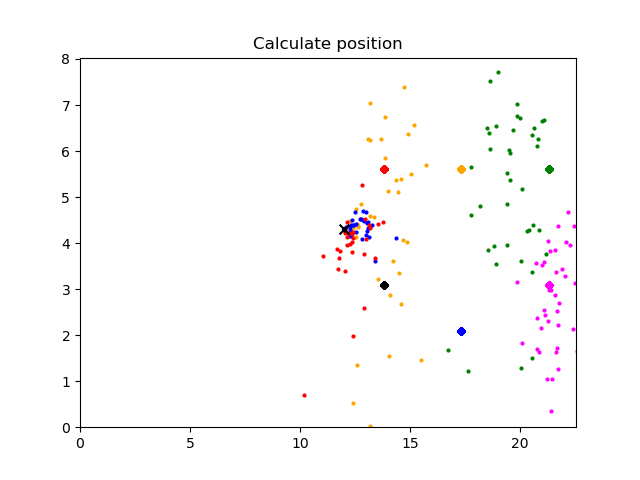
\includegraphics[scale=0.8]{figures/plot_pos.PNG}
		\caption{Représentation des points non convergés par rapport aux positions réelles}
		\label{fig:plotPos} %% NOTE: always label *after* caption!
	\end{center}
\end{figure}

La Figure \ref{fig:plotPos} met en évidence un phénomène qui tend à faire rapprocher les points sur la position du maitre. Cet effet qui se trouve dans le laboratoire où les mesures ont été effectuées complique la reconnaissance de position.

Ci-dessous, une énumeration des couleurs et de la position associée : 
\begin{enumerate}
	\item Couleur verte (SO) : x = 21.30m / y = 5.60m
	\item Couleur jaune (S1)  : x = 17.30m / y = 5.60m
	\item Ccouleur bleue (S2) : x = 17.30m / y = 2.10m
	\item Couleur rose (S3) : x = 21.30m / y = 3.10m
	\item Couleur rouge (S4) : x = 13.80m / y = 5.60m 
	\item Couleur noir (S5) : x = 13.80m / y = 3.10m 
\end{enumerate} 

Comme décrit plus haut, toute une série de tests ont été effectués afin de trouver d'une part les meilleurs paramètre et d'autre part de trouver les caractéristiques les plus probantes. Dans tous les essais realisés, seul trois seront détaillés ci-dessous:cRésultats obtenus en utilisant uniquement les données de "ranging", résultats ontenus en utilisant uniquement les données de position et finalement présentation de la solution retenue qui utilise la mediane, les données "ranging", les quantiles et la variance.

\subsubsection{Résultat en utilisant toutes les données de ranging brutes}
Le premier test qui a été effectué a été de prendre toutes les données brutes des valeurs de ranging. Cela consiste à prendre chacune des mesures des quatre esclaves sur tous les quarantes cannaux et de les mettre les unes à côté des autres pour en créer une caractéristique. Cela est effectué pour chacune des mesures (40 par position).  

La Figure \ref{fig:matPosSxTRaw} présente le résultat obtenu lorsque l'entrainement est fait avec 32 des 40 mesures sur une même position et testé avec les 8 restants. Le résultat obtenu est impressionnant et offre une précision entre 95\% et 100\%. Les position sont très bien reconnues. La variation de pourcentage pour la reconnaissance vient du fait qu'à chaque lancement, le programme exclu 8 autres mesures.

La matrice de confusion représentée est donnée avec des mesures qui ont été faites sur un même point sans bouger l'espion. Le F1-score macro est de 0.9791 et un F1-score micro de 0.9792.  

%Accuracy with optimisation 97.91666666666666 %
%Accuracy 0.9791666666666666
%F1-Score macro : 0.9790849673202615
%F1-Score micro: 0.9791666666666666
\begin{figure}[htp]
	\begin{center}
		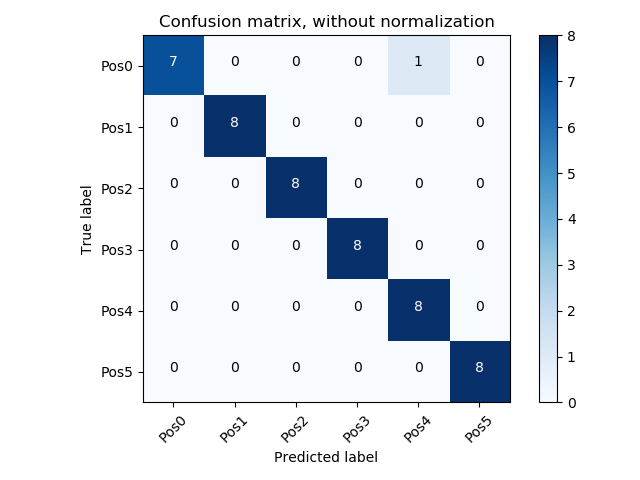
\includegraphics[scale=0.5]{figures/mat_pos_Sx_raw.png}
		\caption{Matrice de confusion obtenue en utilisant les point Sx et les caractéristiques de "ranging"}
		\label{fig:matPosSxTRaw} %% NOTE: always label *after* caption!
	\end{center}
\end{figure}

Afin de valider le système, 5 points suplémentaires par postion ont été pris durant une autre période et en ayant propablement une postion à peine différentes. Il faut précisier que les mesures sur la position 5 ont été effectuées au même moment tant pour les 40 que les 5 mesures. C'est pour cette raison que la détection de cette position est très bonne. 

Cela montre une précision de 46.67\% ce qui correspond à 14 positions correctement reconnues sur 30. Ces résultats ne sont pas encourageant car cela veut dire que sitôt que l'espion est positionné différement mais au même endroit cela influence grandement la reconnaissance. Il est donc nécessaire d'effectuer un travaille supplémentaire pour améliorer cette reconnaissance soit niveau prise de mesure soit niveau du travail sur les caractéristiques. Ce qui a été obtenu dans ce test n'était pas ce qui était attendu au vu des résultats obtenus précédement dans la Figure \ref{fig:matPosSxTRaw}.
%toute les raw
%Accuracy with optimisation 46.666666666666664 %
%Accuracy with optimisation 14 sur 30
%Accuracy 0.4666666666666667
\begin{figure}[htp]
	\begin{center}
		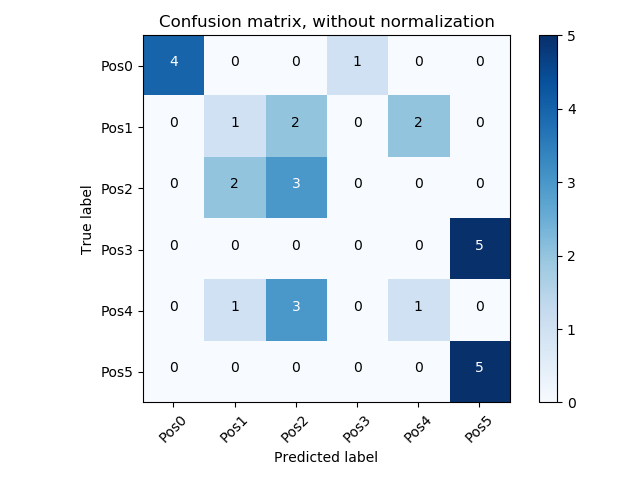
\includegraphics[scale=0.5]{figures/mat_pos_SxT_rawall.png}
		\caption{Matrice de confusion obtenue en utilisant les point de tests SxT et les caractéristiques de "ranging" de la 1ère et 2ème mesures de l'esclave}
		\label{fig:matPosSxTRawall} %% NOTE: always label *after* caption!
	\end{center}
\end{figure}

Deux mesures sont effectuées par esclave pour les quarantes cannaux. L'exemple précédent prend en compte toutes ces mesures. Afin de voir l'effet de ces mesures, un essai a été de prendre uniquement chaque première mesure et ensuite chaque seconde mesure. Etonnement cela à amélioré les résultats comme le montre la Figure \ref{fig:matPosSxTRaw1}. Les premières mesures offre de mauvais résultats alors que prendre uniquement les deuxièmes mesures améliore le score. La précision obtenue est de 53.33\% ce qui correspond à 16 positions correctement reconnues sur 30. Difficile à conclure le pourquoi de cette amélioration, afin de clarifier cette influence il serait intéressant de faire plus de deux mesures et regarder les différents résultats.
%Accuracy with optimisation 53.333333333333336 %
%Accuracy with optimisation 16 sur 30
%Accuracy 0.5333333333333333
\begin{figure}[htp]
	\begin{center}
		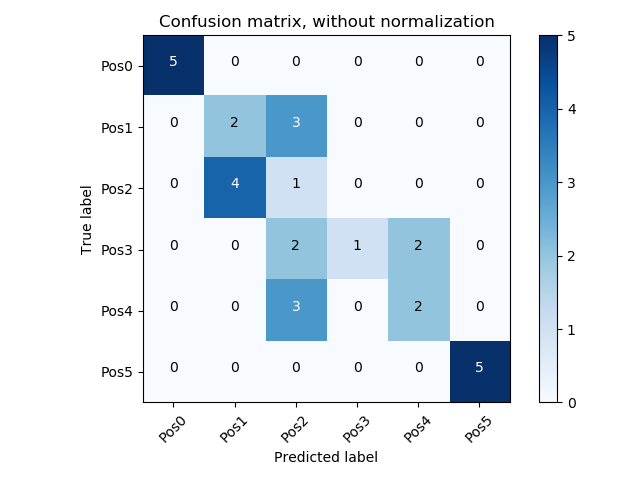
\includegraphics[scale=0.5]{figures/mat_pos_SxT_raw1.png}
		\caption{Matrice de confusion obtenue en utilisant les point de tests SxT et les caractéristiques de "ranging" de la 2ème mesure de l'esclave uniquement}
		\label{fig:matPosSxTRaw1} %% NOTE: always label *after* caption!
	\end{center}
\end{figure}

\subsubsection{Résultat en utilisant la position non convergée}
Le résulat qui est présenté ici permet de faire une comparaison entre une mesure qui est convergée (présenté au chapitre suivant) ou une mesure qui est calculé uniquement à partir de huit mesure. C'est sans surprise que les résultats qui sont obtenus sont vraiment moins bons.

La Figure \ref{fig:matPosSxTPos} présente le résultat obtenu lorsque l'entrainement est fait avec 32 des 40 mesures sur une même position et testé avec les 8 restants. Le résultat obtenu est impressionnant et offre une précision d'environ 70\% contre environ 85\% pour la solution avec les positions convergées. 

La matrice de confusion représentée est donnée avec des mesures qui ont été faites sur un même point sans bouger l'espion. La précision est de 72.91\%, le F1-score macro est de 0.7102 et un F1-score micro de 0.7293.  
%Accuracy with optimisation 72.91666666666666 %
%Accuracy 0.7291666666666666
%F1-Score macro : 0.7102357609710551
%F1-Score micro: 0.7291666666666665
\begin{figure}[htp]
	\begin{center}
		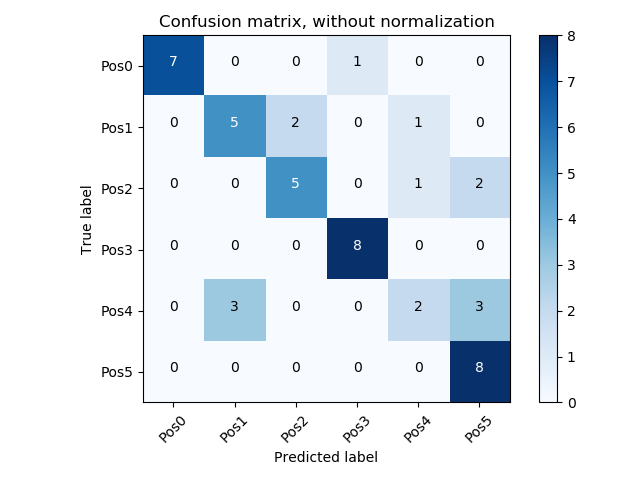
\includegraphics[scale=0.5]{figures/mat_pos_Sx_pos.png}
		\caption{Matrice de confusion obtenue en utilisant les point Sx et la caractéristique de position}
		\label{fig:matPosSxTPos} %% NOTE: always label *after* caption!
	\end{center}
\end{figure}
83.33%

Afin de valider le système, 5 points suplémentaires par postion ont été pris durant une autre période et en ayant propablement une postion à peine différentes. Il faut précisier que les mesures sur la position 5 ont été effectuées au même moment tant pour les 40 que les 5 mesures. C'est pour cette raison que la détection de cette position est très bonne. 

Cela montre une précision de 43.33\% ce qui correspond à 13 positions correctement reconnues sur 30 alors que les résultats pour les positions convergées donnent 83.33\% qui correspond à une reconnaissance correcte de 25 position sur 30.

%Accuracy with optimisation 43.333333333333336 %
%Accuracy with optimisation 13 sur 30
%Accuracy 0.43333333333333335
\begin{figure}[htp]
	\begin{center}
		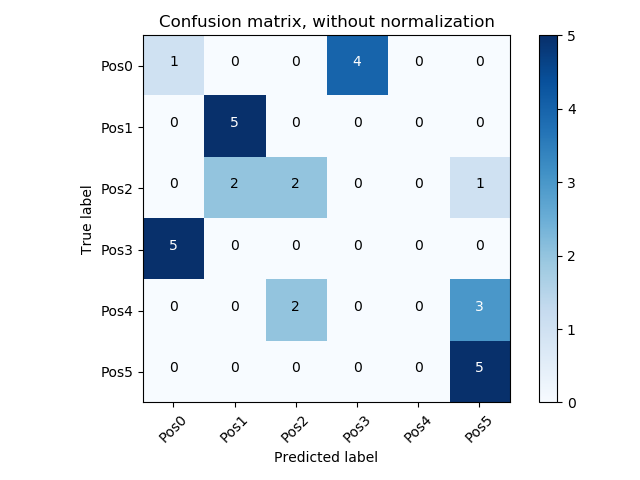
\includegraphics[scale=0.5]{figures/mat_pos_SxT_pos.png}
		\caption{Matrice de confusion obtenue en utilisant les poitns SxT et la caractérisitque de position}
		\label{fig:matPosSxTPos} %% NOTE: always label *after* caption!
	\end{center}
\end{figure}

\subsubsection{Meilleur résultat obtenu}
Ce chapitre va présenter le meilleur résultat qui a été obtenu ainsi que les caractéristiques qui ont été utilisées. Pour y arriver les caractéristiques suivantes ont été testée de manière individuelle :
 
\begin{enumerate}
	\item Toutes les données "ranging" (raw)
	\item Donnée ranfing d'un canal (raw) 
	\item La moyenne des cannaux
	\item La variance sur les cannaux
	\item Déviation standard sur les cannaux
	\item Quantile effectué sur les cannaux
	\item Médiane effectuée sur les cannaux 
	\item Covariance des cannaux
\end{enumerate}

Ensuite, plusieurs association ont été faites entre ses différents test et le meilleur des résultats est obtenu en associant la valeur de la médiane, de la variance, du quantile et des données de "ranging". A noter que pour avoir le meilleur résultat, il a été nécessaire de prendre en compte uniquement la deuxième mesure de ranging sur chaque esclave. Lorsque les différentes caractéristiques sont affichée, il est à noter que l'amplitude des valeurs n'est pas du même ordre et par conséquent pour tenter de les égaliser, la médiane a été multipliée par cinq, le quantile par six et la variance a été divisée par quatre. Cette façon de faire à encore amélioré les résultats pour obtenir ceux présenté ci-dessous

La Figure \ref{fig:matPosSx} présente le résultat obtenu lorsque l'entrainement est fait avec 32 des 40 mesures sur une même position et testé avec les 8 restants. Cela donne de très bonnes précisions qui se situent entre 83\% et 98\%. Les position sont majortiairement bien reconnues. La variation de pourcentage pour la reconnaissance vient du fait qu'à chaque lancement, le programme exclu 8 autres mesures.

La matrice de confusion représentée est donnée avec des mesures qui ont été faites sur une même point sans bouger l'espion. La précision dans ce cas est de 97.92\% avec un F1-score macro de 0.9791 et un F1-score micro de 0.9792. 

\begin{figure}[htp]
	\begin{center}
		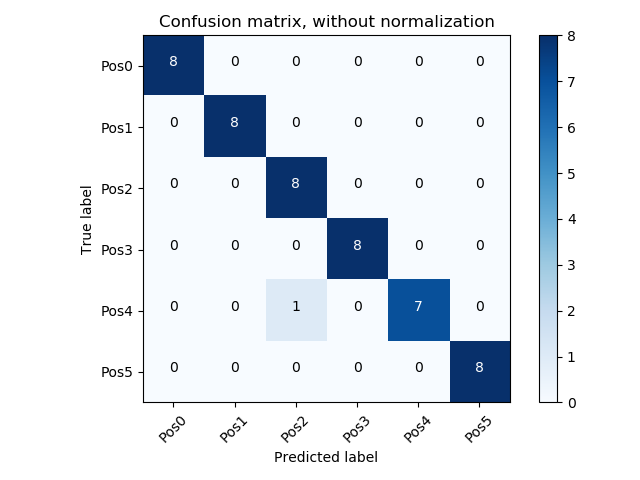
\includegraphics[scale=0.5]{figures/mat_pos_Sx.PNG}
		\caption{Matrice de confusion obtenue pour la meilleures solution en utilisant les données des point Sx}
		\label{fig:matPosSx} %% NOTE: always label *after* caption!
	\end{center}
\end{figure}

Maintenant, afin de valider le système 5 points suplémentaires par postion ont été pris durant une autre période de la journée et en ayant propablement une postion à peine différentes. La présentation des précédents résultat montre de très mauvais résultats concernant ce test mais après le travail effectué et la recherches des meilleures caractéristiques les résultas sont satisfaisants et encourageant. Il faut précisier que les mesures sur la position 5 ont été effectuées au même moment tant pour les 40 que les 5 mesures. C'est pour cette raison que la détection de cette position est très bonne. 

Cela montre une précision de 73.33\% ce qui correspond à 22 positions correctement reconnue sur 30. 
%Accuracy with optimisation 73.33333333333333 %
%Accuracy with optimisation 22 sur 30
%Accuracy 0.7333333333333333
\begin{figure}[htp]
	\begin{center}
		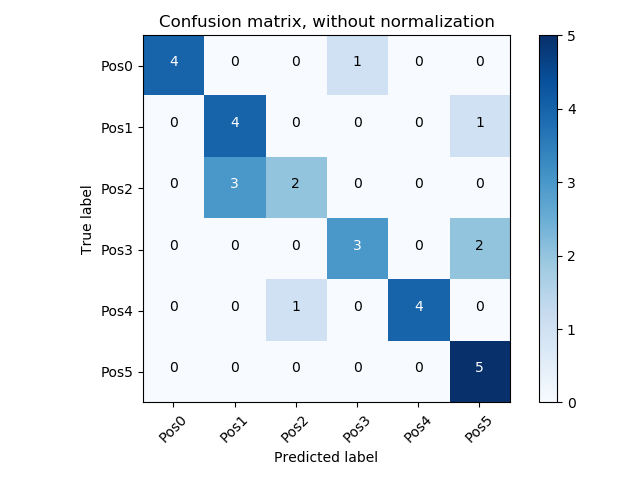
\includegraphics[scale=0.5]{figures/mat_pos_SxT.png}
		\caption{Matrice de confusion pour la meilleures solution en utilisant les point de tests SxT}
		\label{fig:matPosSxT} %% NOTE: always label *after* caption!
	\end{center}
\end{figure}

Un dernier test a été réalisé afin de voir si les positions Tx sont bien reconnue par rapport à leur plus proche voisin. La Figure \ref{fig:matPosTx} montre les résultats obtenus lorsque les positions Tx sont utilisées. Les points T1/2/7/8 correspondent à la position S0, T3/4/9 correspondent à la position S1, T5 correspond à la position S2, T0/6 correspondent à la position S3 et finalement, T10/11/12 correspondent à la position S4. Comme attendu les résultats pour cette classification ne sont pas bons est pas utilisable. La précision obtenue est de 31.25\% ce qui représente une détection correcte de 20 positions sur 64. Pour obtenir ce résultat on essaie de classifier les positions Tx selon la position entrainée la plus proche. 

\begin{figure}[htp]
	\begin{center}
		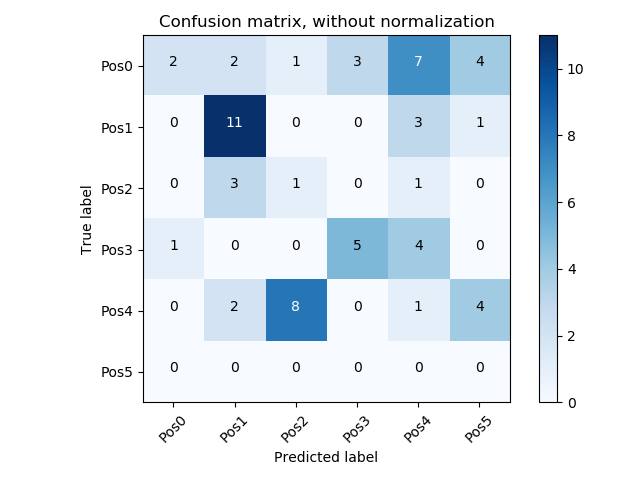
\includegraphics[scale=0.5]{figures/mat_pos_Tx.png}
		\caption{Matrice de confusion pour les valeurs de la position convergée avec des points de tests positionnés autour des points entrainés}
		\label{fig:matPosTx} %% NOTE: always label *after* caption!
	\end{center}
\end{figure}

\subsection{Résultats en utilisant les données de position convergées}
Ce chapitre va présenter les résultats qui ont été obtenus à partir des approximation de position fournies par le programme de mesures. Dans cette partie uniquement ces valeurs seront utilisée. Afin d'avoir une meilleure vue de ce que représente ces positions, la Figure \ref{fig:plotPosConv} montre le positionnement des points calculés par rapport à la position réelle de l'espion. Les gros points de couleurs représentent la position réelle et les petits points de couleurs représentent les positions calculées. La croix noir représente la position du master. 

\begin{figure}[htp]
	\begin{center}
		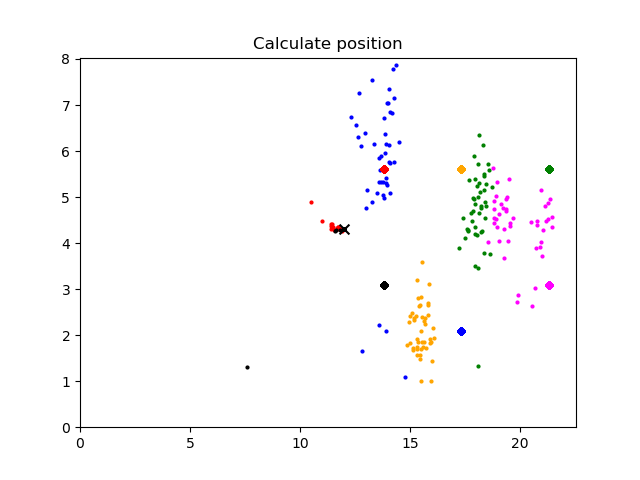
\includegraphics[scale=0.8]{figures/plot_pos_conv.PNG}
		\caption{Représentation des points convergés par rapport aux positions réelles}
		\label{fig:plotPosConv} %% NOTE: always label *after* caption!
	\end{center}
\end{figure}

La Figure \ref{fig:plotPosConv} met en évidence un phénomène qui tend à faire correspondre les points proches du maitre sur les coordonnées du maitre. Cet effet qui se trouve dans le laboratoire où les mesures ont été effectuées complique la reconnaissance de position. De par cette représentation, il est possible de voir à l'oeil nu la séparation des points par contre, il est rapidement possible de se rendre compte que si on ajoute des points il sera de plus en plus difficile à différencier les emplacements de base de l'espion.

Ci-dessous, une énumeration des couleurs et de la position associée : 
\begin{enumerate}
	\item Couleur verte (SO) : x = 21.30m / y = 5.60m
	\item Couleur jaune (S1)  : x = 17.30m / y = 5.60m
	\item Ccouleur bleue (S2) : x = 17.30m / y = 2.10m
	\item Couleur rose (S3) : x = 21.30m / y = 3.10m
	\item Couleur rouge (S4) : x = 13.80m / y = 5.60m 
	\item Couleur noir (S5) : x = 13.80m / y = 3.10m 
\end{enumerate} 

La Figure \ref{fig:matPosConvSx} représente le résultat obtenu lorsque l'entrainement est fait avec 32 des 40 mesures sur une même position et testé avec les 8 restants. Cela donne de très bonnes précisions qui se situent entre 81\% et 89\%. Comme attendu, les positions proches du maitre (S4 et S5) se confondent et pas conséquent ne sont pas correctement reconnues. Les autres position sont majortiairement bien reconnu à l'exception de quelques mesures. La variation de pourcentage pour la reconnaissance vient du faire qu'à chaque lancemnt, le programme exclu 8 autres mesures.

\begin{figure}[htp]
	\begin{center}
		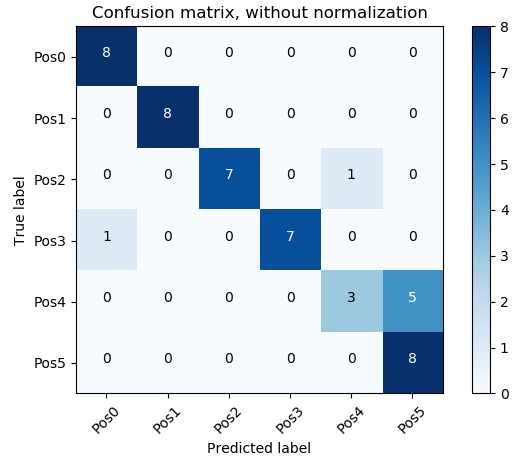
\includegraphics[scale=0.5]{figures/mat_pos_conv_Sx_2.PNG}
		\caption{Matrice de confusion pour les valeurs de la position convergée avec des points positionnés à la même place}
		\label{fig:matPosConvSx} %% NOTE: always label *after* caption!
	\end{center}
\end{figure}

Afin de tester l'algorithme fixé, il est entrainé avec les 40 mesures effectuée sur chaque position de l'espion. Ces 40 mesures sont celles utilisée pour définir les meilleurs paramètres et obtenir les meilleurs résultats comme présenté dans la Figure \ref{fig:plotPosConv}. La Figure \ref{fig:matPosConvSxT} présente le resultat final obtenu avec les cinq données de test qui avaient été effectué à la même position que les quarante de l'entrainement. 

La précision obtenue pour ce test est de 83.33\% ce qui correspond à une reconnaissance correcte de 25 position sur 30. Les positions mal reconnue sont sans surprise les positions S4 et S5.

\begin{figure}[htp]
	\begin{center}
		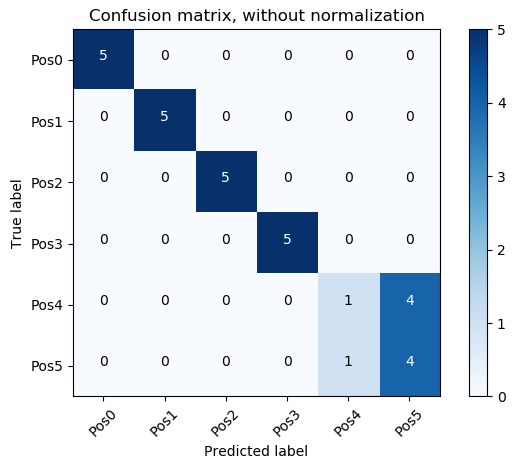
\includegraphics[scale=0.5]{figures/mat_pos_conv_SxT.png}
		\caption{Matrice de confusion pour les valeurs de la position convergée avec des points de tests positionnés à la même place}
		\label{fig:matPosConvSxT} %% NOTE: always label *after* caption!
	\end{center}
\end{figure}

La Figure \ref{fig:matPosConvTx} montre les résultats obtenus lorsque les positions Tx sont utilisées. Les points T1/2/7/8 correspondent à la position S0, T3/4/9 correspondent à la position S1, T5 correspond à la position S2, T0/6 correspondent à la position S3 et finalement, T10/11/12 correspondent à la position S4. Comme attendu les résultats pour cette classification n'est pas bonne est pas utilisable. La précision obtenue est de 21.67\% ce qui représente une détection correcte de 13 position sur 60. Pour obtenir se résultat on essaie de classifier les positions Tx selon la position entrainée la plus proche. 

\begin{figure}[htp]
	\begin{center}
		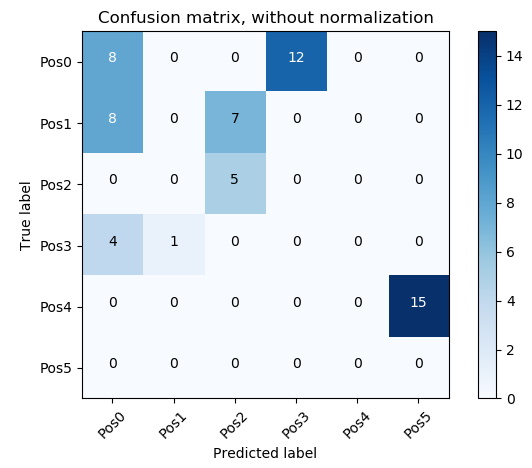
\includegraphics[scale=0.5]{figures/mat_pos_conv_Tx.png}
		\caption{Matrice de confusion pour les valeurs de la position convergée avec des points de tests positionnés autour des points entrainés}
		\label{fig:matPosConvTx} %% NOTE: always label *after* caption!
	\end{center}
\end{figure}

\section{Résumé des résultats}

\begin{figure}[htp]
	\begin{center}
		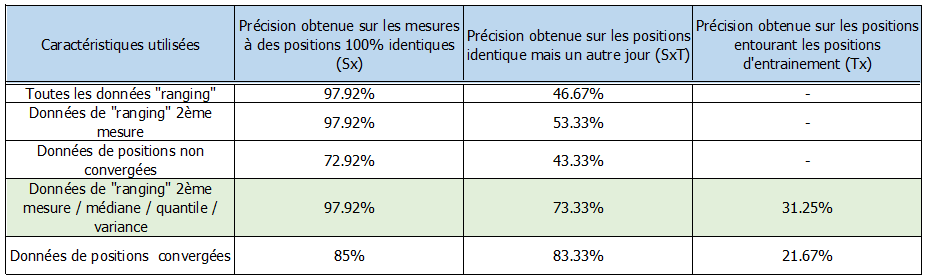
\includegraphics[scale=0.5]{figures/Resultats.png}
		\caption{Résumé des différents résultats obtenus qui sont présentés dans ce rapport}
		\label{fig:result} %% NOTE: always label *after* caption!
	\end{center}
\end{figure}


\chapter{Problèmes rencontrés et améliorations}

%\begin{lstlisting}
% for i=0 to Array.length(t)-1 do
%\end{lstlisting}


%\begin{enumerate}
%	\item fgfd
%	\item gdgfd
%\end{enumerate}


%\begin{figure}[H]
%	\begin{center}
%		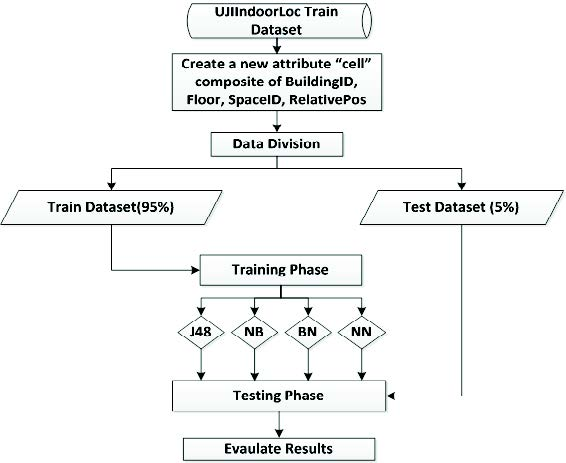
\includegraphics[scale=1]{figures/newattribute.jpg}
%		\caption{The new attribute “cell” construction phase}
%		\label{fig:newAttribute} %% NOTE: always label *after* caption!
%	\end{center}
%\end{figure}

%\todo{Compléter cette partie qui semble importante}

